\documentclass[a4paper,fleqn,usenatbib]{mnras}

%=========================================================================
\usepackage{amsmath} 
\usepackage{amssymb} 
\usepackage{graphicx}
\usepackage{grffile}
\usepackage[dvips]{epsfig}
\usepackage{epsfig}  
\usepackage{color}
\usepackage{caption}
\usepackage{hyperref}
\usepackage{bm}
%Non reposionated tables




%=========================================================================
%		INTERNAL MACROS
%=========================================================================
\def\be{\begin{equation}}
\def\ee{\end{equation}}
\def\ba{\begin{eqnarray}}
\def\ea{\end{eqnarray}}

% To highlight comments 
\definecolor{red}{rgb}{1,0.0,0.0}
\newcommand{\red}{\color{red}}
\definecolor{darkgreen}{rgb}{0.0,0.5,0.0}
\newcommand{\SRK}[1]{\textcolor{darkgreen}{\bf SRK: \textit{#1}}}
\newcommand{\SRKED}[1]{\textcolor{darkgreen}{\bf #1}}
\newcommand{\before}[1]{\textcolor{red}{ #1}}
\newcommand{\after}[1]{\textcolor{darkgreen}{ #1}}
\newcommand{\hs}{{\hspace{1mm}}}  
\newcommand{\tol}{Tololo 1214-277}
\newcommand{\rank}{\texttt{Ranked}}
\newcommand{\boot}{\texttt{Bootstrapped}}
\newcommand{\rand}{\texttt{Random}}
\newcommand{\HI}{{\text{H\MakeUppercase{\romannumeral 1}}} }
\newcommand{\HII}{{\text{H\MakeUppercase{\romannumeral 2}}} }
\newcommand{\lya}{\ifmmode{{\rm Ly}\alpha}\else Ly$\alpha$\ \fi}
\newcommand{\cm}{\ifmmode{{\rm cm}}\else cm\fi}
\newcommand{\ccm}{\,\mathrm{cm}^{-3}}
\newcommand{\ergps}{\,{\rm erg}\,{\rm s}\ifmmode{}^{-1}\else ${}^{-1}$\fi}
\newcommand{\Mpch}{\,{\rm Mpc}\,\ifmmode h^{-1}\else $h^{-1}$\fi}
\newcommand{\dd}{\mathrm{d}}
\newcommand{\vek}[1]{\bm{#1}}
\newcommand{\hb}{H$\beta$}
\newcommand{\ha}{H$\alpha$}
\newcommand{\oiii}{[OIII]}
\newcommand{\oii}{[OII]}
\newcommand{\nii}{[NII]}
\newcommand{\esca}{erg cm$^{-2}$ s$^{-1}$ \AA$^{-1}$}
\newcommand{\esc}{erg cm$^{-2}$ s$^{-1}$}
\newcommand{\es}{erg s$^{-1}$}
\newcommand{\esa}{erg s$^{-1}$}
\newcommand{\kms}{\ifmmode\mathrm{km\ s}^{-1}\else km s$^{-1}$\fi}
\newcommand{\hMsun}{{\ifmmode{h^{-1}{\rm{M_{\odot}}}}\else{$h^{-1}{\rm{M_{\odot}}}$}\fi}}
\newcommand{\Msun}{{\ifmmode{{\rm{M_{\odot}}}}\else{${\rm{M_{\odot}}}$}\fi}}

\newcommand{\jefr}[1]{\textcolor{darkgreen}{\bf JEFR: \textit{#1}}}

\begin{document}

%=========================================================================
%		FRONT MATTER
%=========================================================================
\title[No Title]{No Title}
\author[J.E. Forero-Romero \& V. Arias]
{Jaime E. Forero-Romero $^{1}$ \thanks{je.forero@uniandes.edu.co},
Ver\'onica Arias$^1$\\
%%
$^1$ Departamento de F\'isica, Universidad de los Andes, Cra. 1
  No. 18A-10 Edificio Ip, CP 111711, Bogot\'a, Colombia \\
}

\maketitle

\begin{abstract}
We quantify the joint spatial distribution of the brightest satellites
around the Milky way and M31. 
We find that the satellites in MW show a distribution significantly
thinner and flattened compared to the expectaions of a random
spherical distribution and simulations based on the Lambda Cold Dark
Matter paradigm.
In turn, M31 is completely consistent with the expectations from a
spherical satellite distribution and LCDM simulations.
The satellite planes in the MW and M31 are almost perpendicular to the line
connecting the two galaxies. None of the pairs in the simulation show
a similar degree of alignment. 
However, the simulations are consistent with a random uniform
distribution, making the result from the observations consistent with
these theoretical expectations.
This special satellite distribution in the Milky Way makes the Local
Group an atypical pair in the cosmological context provided by
simulations. 
We summarize these results in a simple multivariate Gaussian
model to estimate that only $1\%$ of the pairs with isolation
and dynamical characteristics similar to the LG are expected to have
satellite distributions with the same degree of atipicality. 
\end{abstract}

\begin{keywords}Galaxies: halos --- Galaxies: high-redshift --- Galaxies: statistics
--- Dark Matter --- Methods: numerical 
\end{keywords}

\section{Introduction}

 
It has been shown that LG pair separation vector is aligned along the
filaments in  which they are typically embeded
\cite{2015ApJ...799...45F}, the LG pairs found in pancake-like DM
matter arrangements are aligned with the plane itself. 
Characterizing the satellite alignments with $\mu$ thus provide
information about how satellites are distributed with respect to the
cosmic web. 

In Section we list the sources of the observational and
simulated data to be used throughout the paper.
Next, in Section we describe the methods we use to quantify and
characterize the satellite distributions.
In section we present our results. 
In the discussion section we quantify the correlations between the main
plane properties as described by the simulations.
We use this results to quantify the degree of atipicality of the LG
and estimate the volume that has to probed in simulations in order to
find a pair with a satellite distribution as atipical as the LG. 
Finally, we summarize our conclusions in Section .


\section{Observational Data}
\label{sec:obs}


\section{Local Group Satellites in the Illustris Simulation}
\label{sec:NumericalSetup}

We use publicly available data from the Illustris Project 
\citep{2014MNRAS.444.1518V}. 
This suite of cosmological simulations, performed using the quasi-Lagrangian
code AREPO \citep{2010MNRAS.401..791S}, followed the coupled evolution of dark 
matter and gas and includes parametrizations to account for the effects of
gas cooling, photoionization, star formation, stellar feedback, black
hole and super massive black hole feedback. 
The simulation volume is a cubic box of $75$ \Mpch\ on a side.
The cosmological parameters correspond to a $\Lambda$CDM cosmology
consistent with WMAP-9 measurements \citep{2013ApJS..208...19H}. 

We extract halo and galaxy information from the Illustris-1 simulation
which has the highest resolution in the current release of the
Illustris Project.
Illustris-1 has $1820^3$ dark matter particles and $1820^3$ initial gas
volumen elements. 
This corresponds to a dark matter particle mass of
$6.3\times 10^6$\Msun\ and a minimum mass for the baryonic volume
element of $8.0\times 10^7$\Msun. 
The corresponding spatial resolution is $1.4$ kpc for the dark matter
gravitational softening and $0.7$ kpc for the typical size of the
smallest gas cell size. 

We buid a sample of Isolated Pairs that resemble the conditions
in the LG.
To construct this sample we select first all galaxies with  an stellar mass in the range $1\times10^{10}\Msun
<M_{\star}<1.5 \times 10^{11} \Msun$.
Then we consider the following criteria for all galaxies in that set.


\begin{itemize}
\item For each galaxy $A$ we find its closest galaxy $B$, if galaxy $A$ is also
the closest to halo $B$, the two are considered as a pair. 
\item With $d_{AB}$ the distance between the two galaxies and
  $M_{\star,min}$ the lowest stellar mass in the two galaxies, we
  discard pairs that have any other galaxy $C$ with stellar mass
  $M_{\star}>M_{\star, min}$ closer than $3\times d_{AB}$ from any of
  the pair's members. 
\item The distance $d_{AB}$ is greater than $700$ kpc.
\item The relative radial velocity between the two galaxies, including
  the Hubble flow, is $-120\ \kms <v_{AB,r}<0\ \kms$. 
\end{itemize}

We find 27 pairs with these conditions. We show in the Appendix A the
physical  properties (stellar masses, maximum circular velocities,
radial velocities and separation) in those pairs. 
We then select the pairs where in both halos there are at least 15
detected subhalos. 
We end up with a total of 20 pairs that fulfill these criteria. 

Although Illustris-1 has stellar particles, we do not use their
properties to select the satelite population because the smallest
galaxies are barely resolved in stellar mass at magnitudes of
$M_V=9$. We prefer using the dark matter information as the smallest
sub-halos are sampled with $100$ particles. 
For this reason we select the satellite galaxy samples from the

We chose the satellite samples by ranking the subhalos in decreasing
order of its maximum circular velocity and select the first $N_p$
halos in the list. 
The results in the main body of the paper correspond to $11\leq
N_p\leq 15$. 


\section{Satellite Spatial Distribution}
\label{sec:SpatialMeasurements}

We base all our results on the description provided by the inertia
tensor defined by the satellites's positions.  

\begin{equation}
{\bf{\bar{I}}} = \sum_{k \in V}[(\bf{r}_i - \bf{r}_0)^2\cdot \bf{1} -
  (\bf{r}_i-\bf{r}_0)\cdot (\bf{r}_i - \bf{r}_0)^{T}],
\end{equation}
%
where $k$ indexes the set of satellites of interest
$\bf{r}_k$ are the satellites' positions, $\bf{r}_{0}$ is the location
of the central galaxy $\bf{1}$ is the unit matrix,  and  
${\bf r}^T$ is the transposed vector $\bf{r}$. 
We use $\bf{r}_0$ as the position of the central galaxy, and not the
satellites' geometrical center, to allow for a fair comparison once
the angular positions of the satellites are randomized around this
point. 

From this tensor we compute its eigenvalues,
$\lambda_1>\lambda_2>\lambda_3$, and corresponding eigenvectors,
$\hat{I}_1$, $\hat{I}_2$, $\hat{I}_3$.
We define the size of the three ellipsoidal axis as
$a=\sqrt{\lambda_1}$, $b=\sqrt{\lambda_2}$ and $c=\sqrt{\lambda_3}$.
We also define $\hat{n}\equiv \hat{I}_1$ as the vector perpendicular to the
planar satellite distribution. 
We also define the width, $w$, of the planar satellite distribution,
$\sigma_p$ as the standard deviation of all satellite distances to the
plane defined by the vector $\hat{n}$. 
Finally, we characterize the alignment between the satellite plane and the
vector connecting the two dominant galaxies by $\mu=|\hat{r}_{AB}\cdot
\hat{n}|$.

To summarize we characterize the satellite distribution by for
quantities obtained from the inertia tensor: 
\begin{itemize}
\item Plane width, $w$.
\item $c/a$ axis ratio.
\item $b/a$ axis ratio.
\item $\mu$ as a measure of plane alignment.
\end{itemize}


\subsection{Satellite samples}

We compare the satellite distributions in the MW and M31 at fixed
satellite number.
This means that the magnitude cut corresponding to the faintest
satellite included in the sample is different in each case.
We make this choice for two reasons. 
First to always be sure that there is a non-zero number of satellites to make the computations. 
Second, to be able to compare the two halos at a fixed number of
satellites. 

We test the shape and alignment statistics for 11 up 15 satellites.
The lowest number corresponds to the number of classical Milky Way
satellites.
The upper limit corresponds to the minimum number of satellites that
can be resolved in the simulations for both halos in each pair. 
In the case of simulations we rank the subhalos by their maximum
circular velocity. 
We do not use their stellar properties because this represents the
lower resolution limit for the hydrodynamics; most of these subhalos
only have one stellar particle belonging to them. 
In contrast, the detected sub-halos have at least 35 dark matter
particles to determine their properties.


We build two different kinds of statistics from these satellites
First, we compute the shape and alignments for a varying number of
satellites $11\leq N_{s}\leq 15$ keeping their ranking in
$M_V$ or $V_{max}$. 
This allows us to estimate the variation expected by changing the
satellite number. 
The second kind of statistics are computed for a fixed number of
satellites $N_{s}=11$ randomly selected from the top $15$ ranked
satellites. 
We perform this bootstrapping $5$ times for each pair. 
This allows us to estimate the variation expected by randomly sampling
the satellites from a parent distribution.





% referencia posiciones satellites
% http://adsabs.harvard.edu/abs/2013MNRAS.435.1928P

\begin{figure*}
\centering
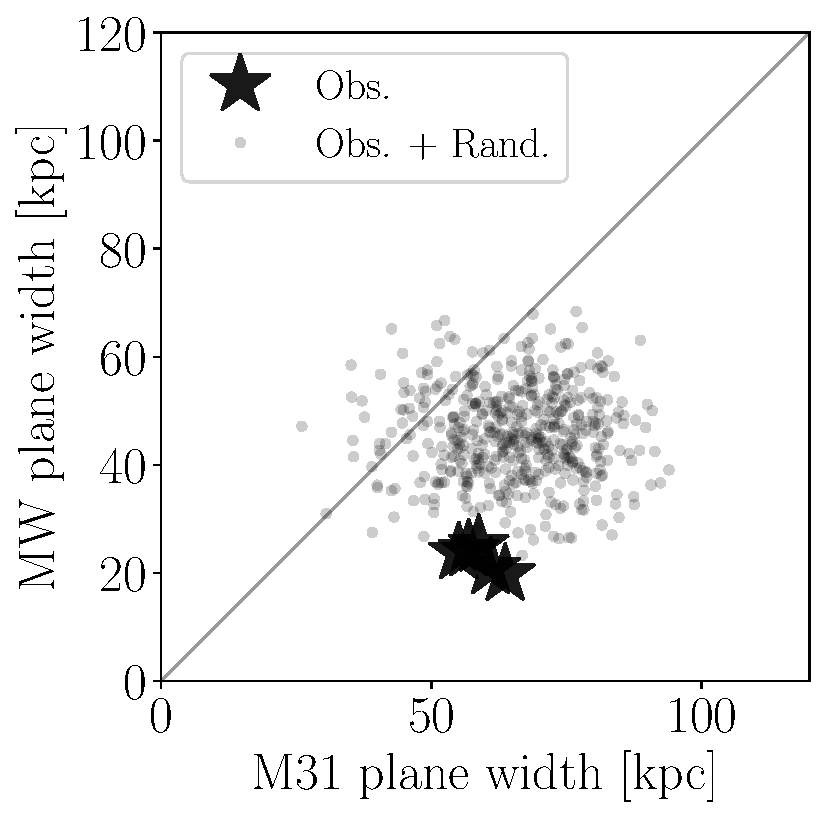
\includegraphics[width=0.32\textwidth]{scatter_random_ranked_width.pdf}
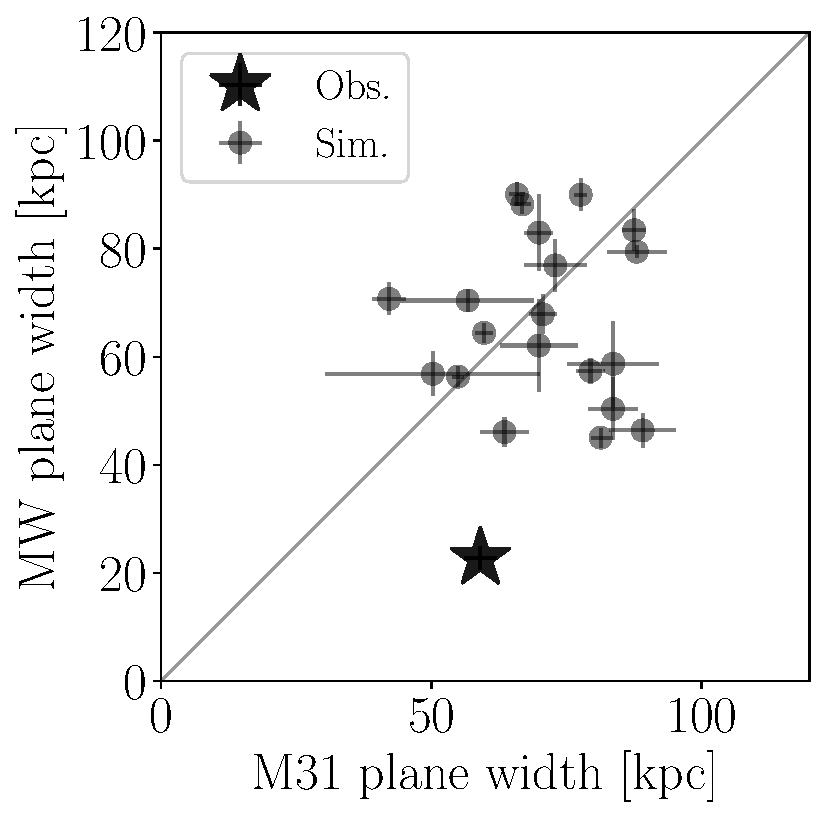
\includegraphics[width=0.32\textwidth]{scatter_ranked_width.pdf}
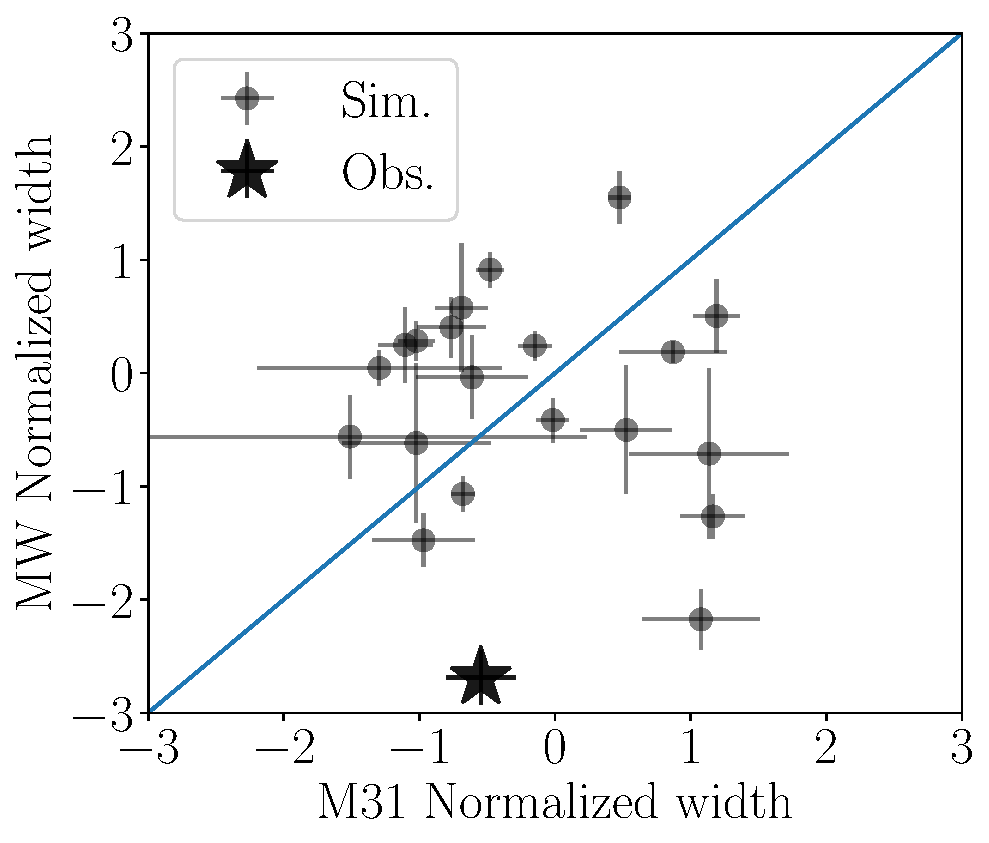
\includegraphics[width=0.32\textwidth]{scatter_norm_width.pdf}
\caption{Plane width characterization in the Local Group and the
  Isolated Pairs. In all panels the horizontal axis corresponds to the
  M31 or the most massive halo in the pair and the vertical axis to
  the MW or the least massive halo in the pair.
The panel on the left shows the plane width in physical units
comparing the results of five measurements from the observations
(stars) and the result of spherically randomizing the satellite
positions (circles). 
The panel in the middle compares the average from the observations
(star) and the average from each one of the Isolated Pairs (circles
with error bars).
The panel on the right has the same information as the middle panel,
only that this time each point has been normalized (median substracted
and normalized by the standar deviation) to the results of its
randomization. 
The main message of this series of plots is that the MW has a
significantly thiner plane both compared to the result of its own
satellite spherical randomization (left panel) and the expectation from
simulations (middle panel). 
This low value is $2\sigma$ away from what is expected in a spherical
distribution. 
In the M31 their satellites are in agreement with the expectations
both from an spherical distribution and the results form the
simulations. 
A second conclusion is that the spherically averaged plane width
MW (seen in the point cloud in the left panel) is smaller than the
average expectation from simulations, while for M31 the spherical
average is consistent with simulations. 
\label{fig:scatter_width}}
\end{figure*}

\begin{figure*}
\centering
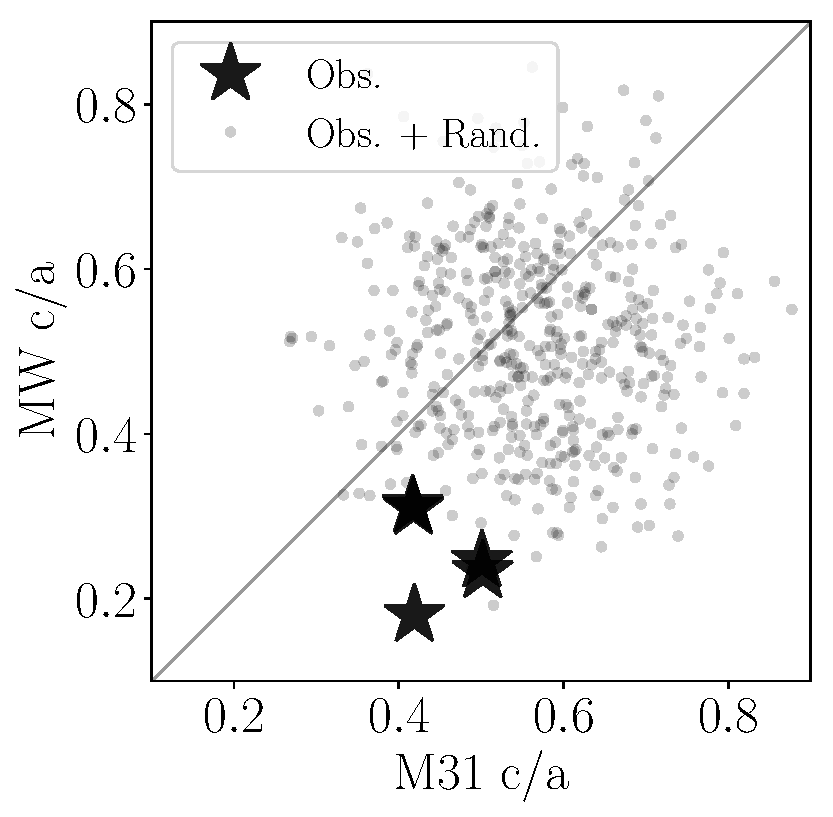
\includegraphics[width=0.32\textwidth]{scatter_random_ranked_ca_ratio.pdf}
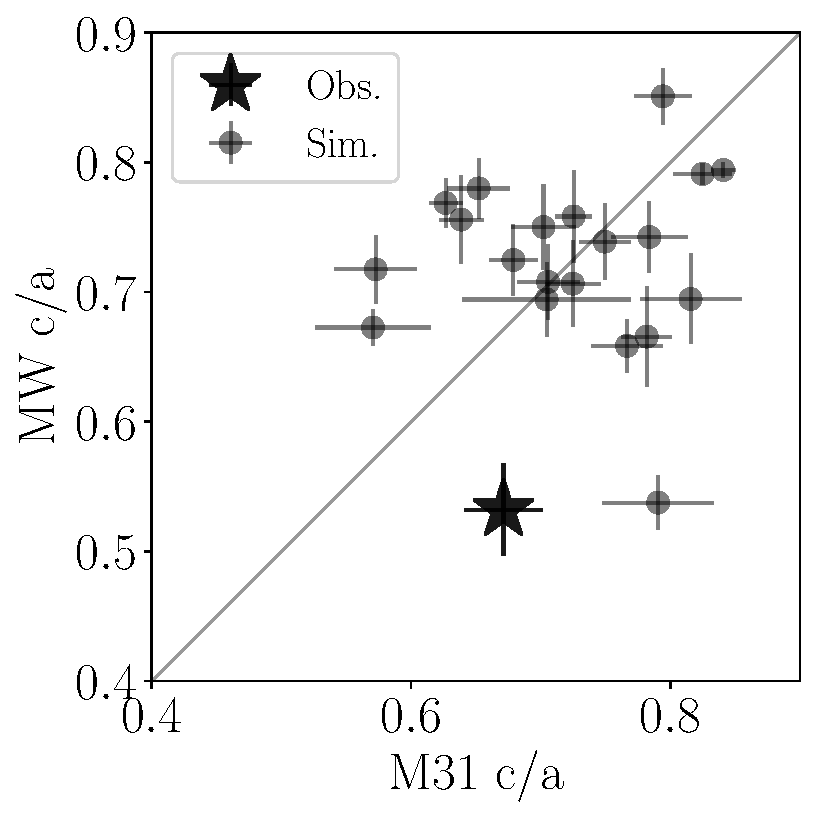
\includegraphics[width=0.32\textwidth]{scatter_ranked_ca_ratio.pdf}
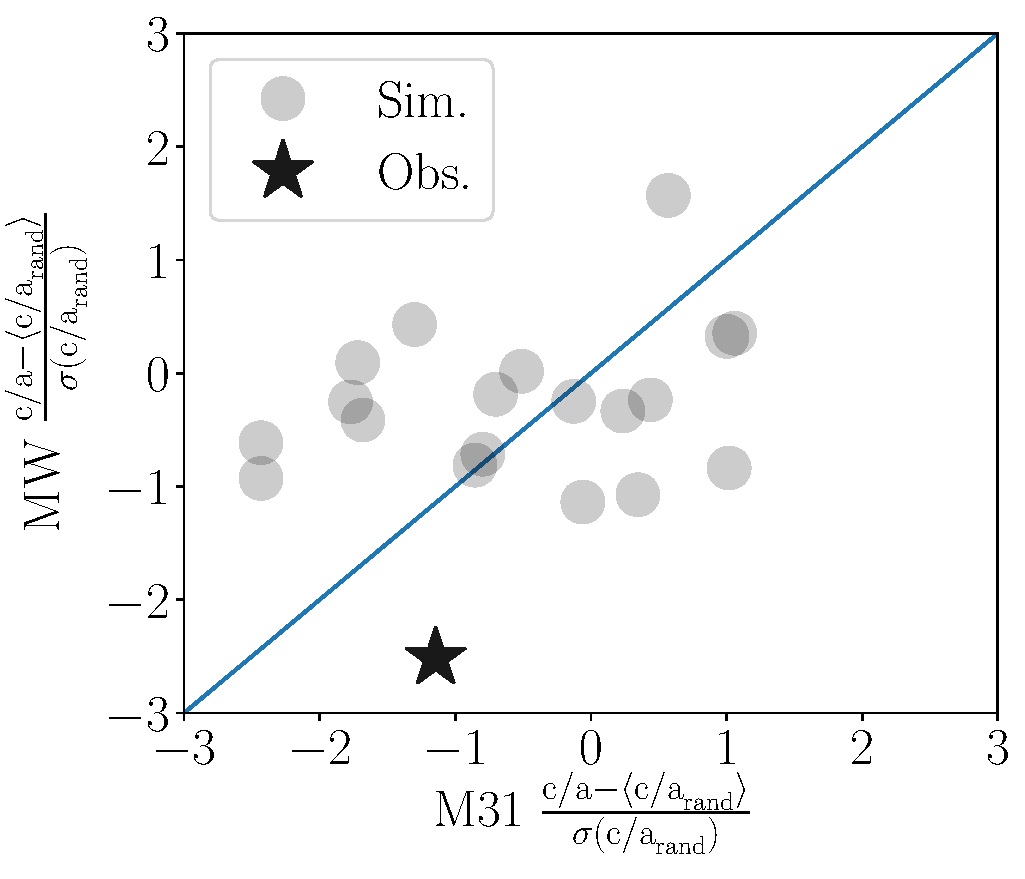
\includegraphics[width=0.32\textwidth]{scatter_norm_ca_ratio.pdf}
\caption{Same layout as in Figure \ref{fig:scatter_width}. 
This time for the $c/a$ axis ratio. 
The message holds in this case as for the plane width.
The MW is has a significantly low $c/a$ value compared to the
expectation from a spherical distribution and simulations. 
This low value is also $2\sigma$ away from the expactations for an
spherical distribution.
M31 is consistent both with an spherical distribution and the results
from simulations.
However, in this case the axis ratio in the spherically averaged case
is completeley consistent with the expectation from simulations.
\label{fig:scatter_ca_ration}}
\end{figure*}


\begin{figure*}
\centering
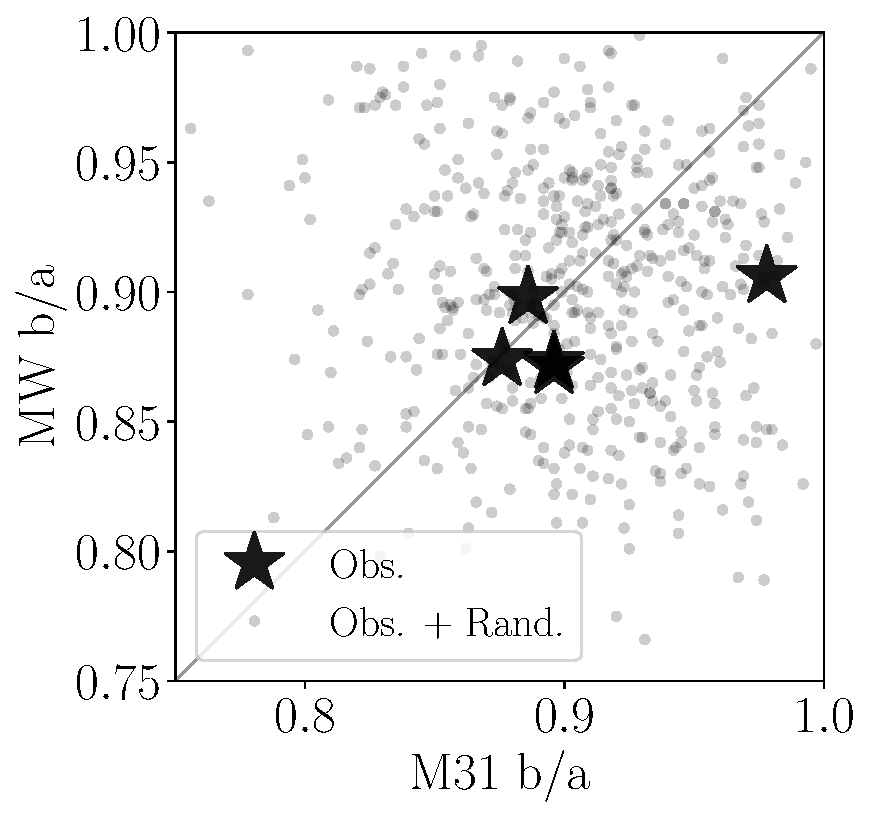
\includegraphics[width=0.32\textwidth]{scatter_random_ranked_ba_ratio.pdf}
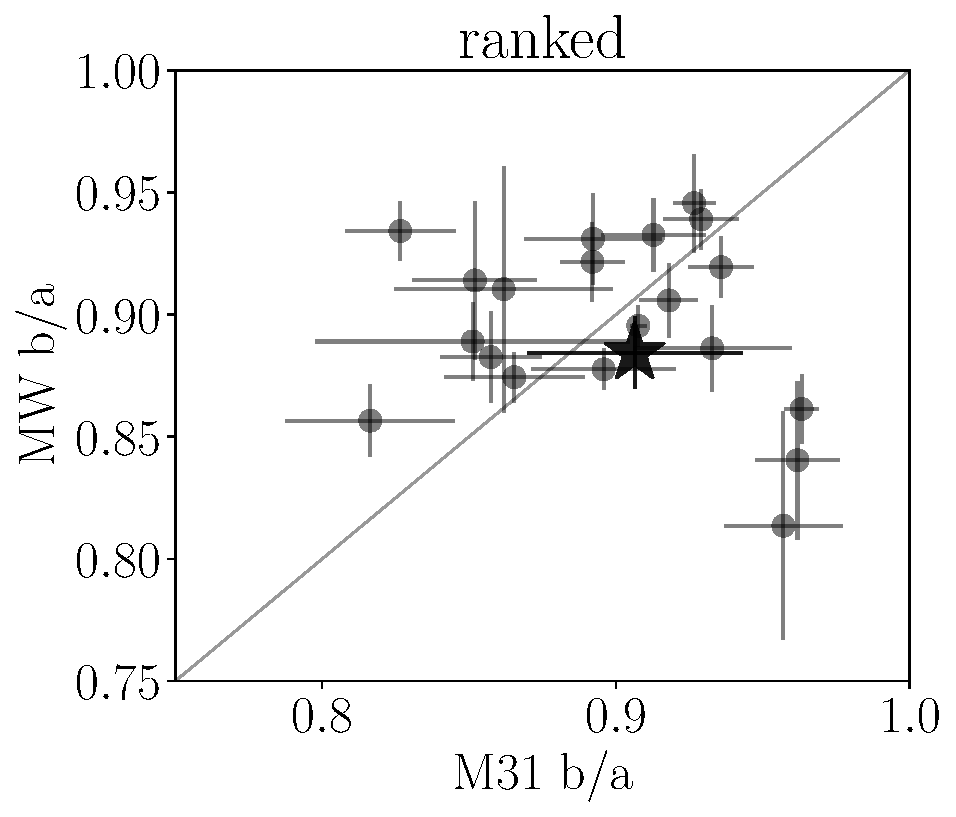
\includegraphics[width=0.32\textwidth]{scatter_ranked_ba_ratio.pdf}
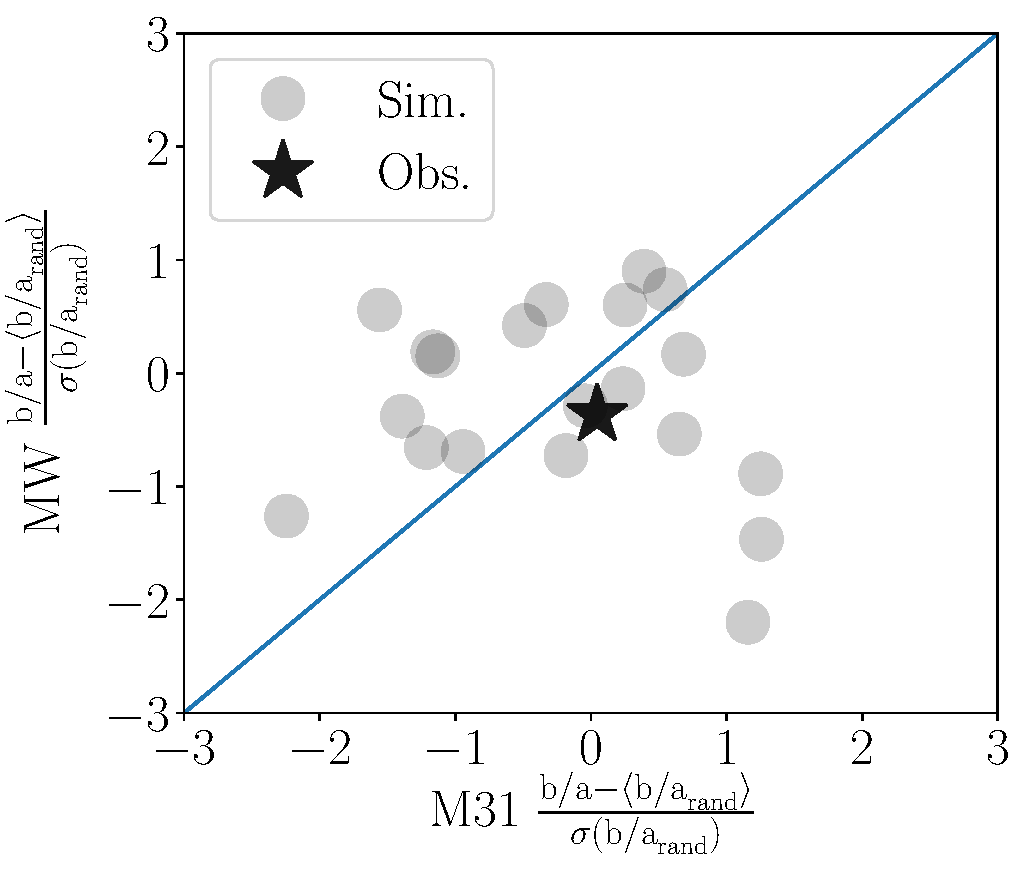
\includegraphics[width=0.32\textwidth]{scatter_norm_ba_ratio.pdf}
\caption{Same layout as in Figure \ref{fig:scatter_width}. 
This time for the $b/a$ axis ratio. In this case both the MW and M31
are consistent with the results of a spherical distribution and the
simulations. 
\label{fig:scatter_ba_ration}}
\end{figure*}

\begin{figure*}
\centering
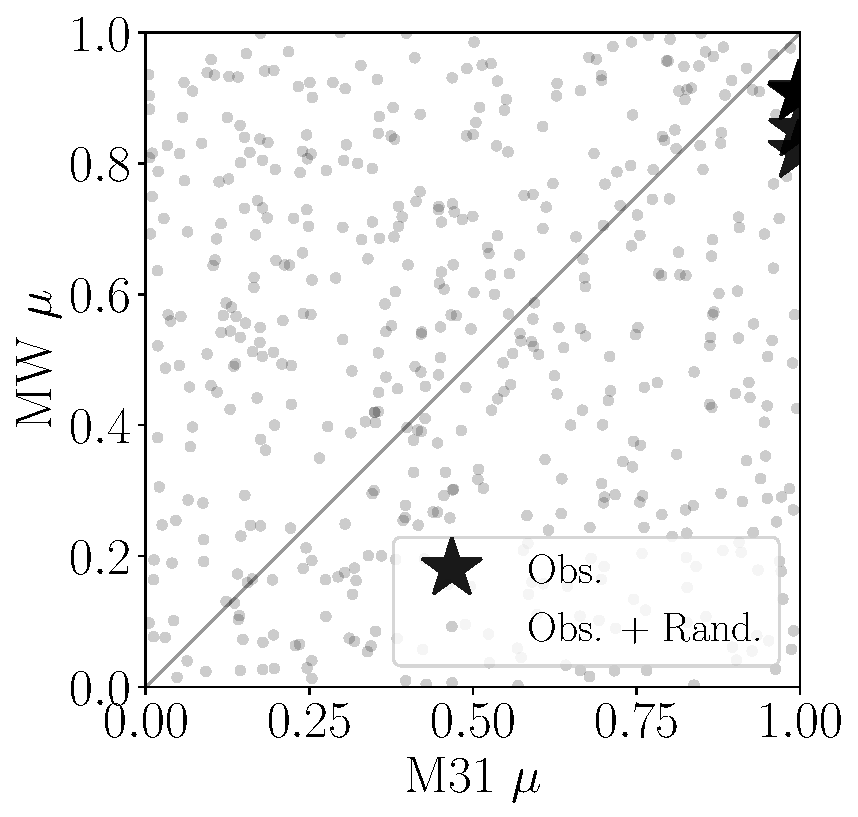
\includegraphics[width=0.32\textwidth]{scatter_random_ranked_mu.pdf}
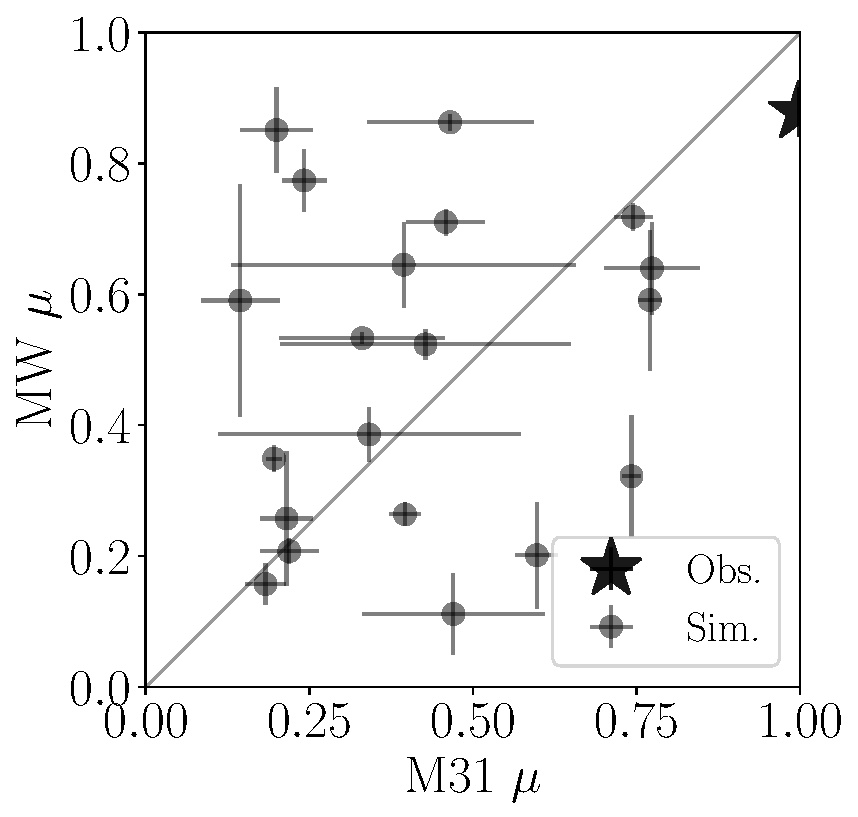
\includegraphics[width=0.32\textwidth]{scatter_ranked_mu.pdf}
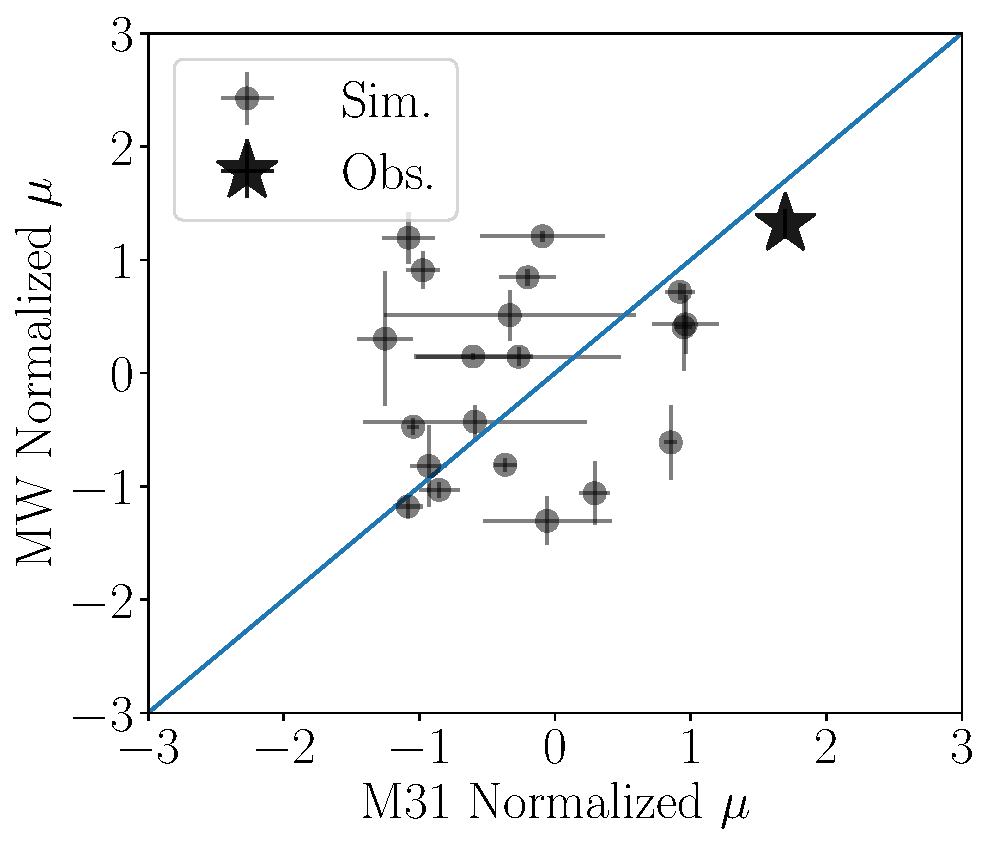
\includegraphics[width=0.32\textwidth]{scatter_norm_mu.pdf}
\caption{Same layout as in Figure \ref{fig:scatter_width}. 
This time for $\mu$ the absolute value of the dot product between the
vector connecting the main galaxies and the vector perpendicular to
the satellite plane.
In this case both the MW and M31 show a strong alignment.
Apparently this result is outside the expectations from the
simulations and atypical compared to the spherical results. 
However, this is not the case. The $\mu$ distributions in the
randomization and the simulation are consistent with a uniform
distribution.
Under such circumstances $\mu\approx 1$ is as likely as
any other value.
\label{fig:scatter_mu}}
\end{figure*}


\begin{figure*}
\centering
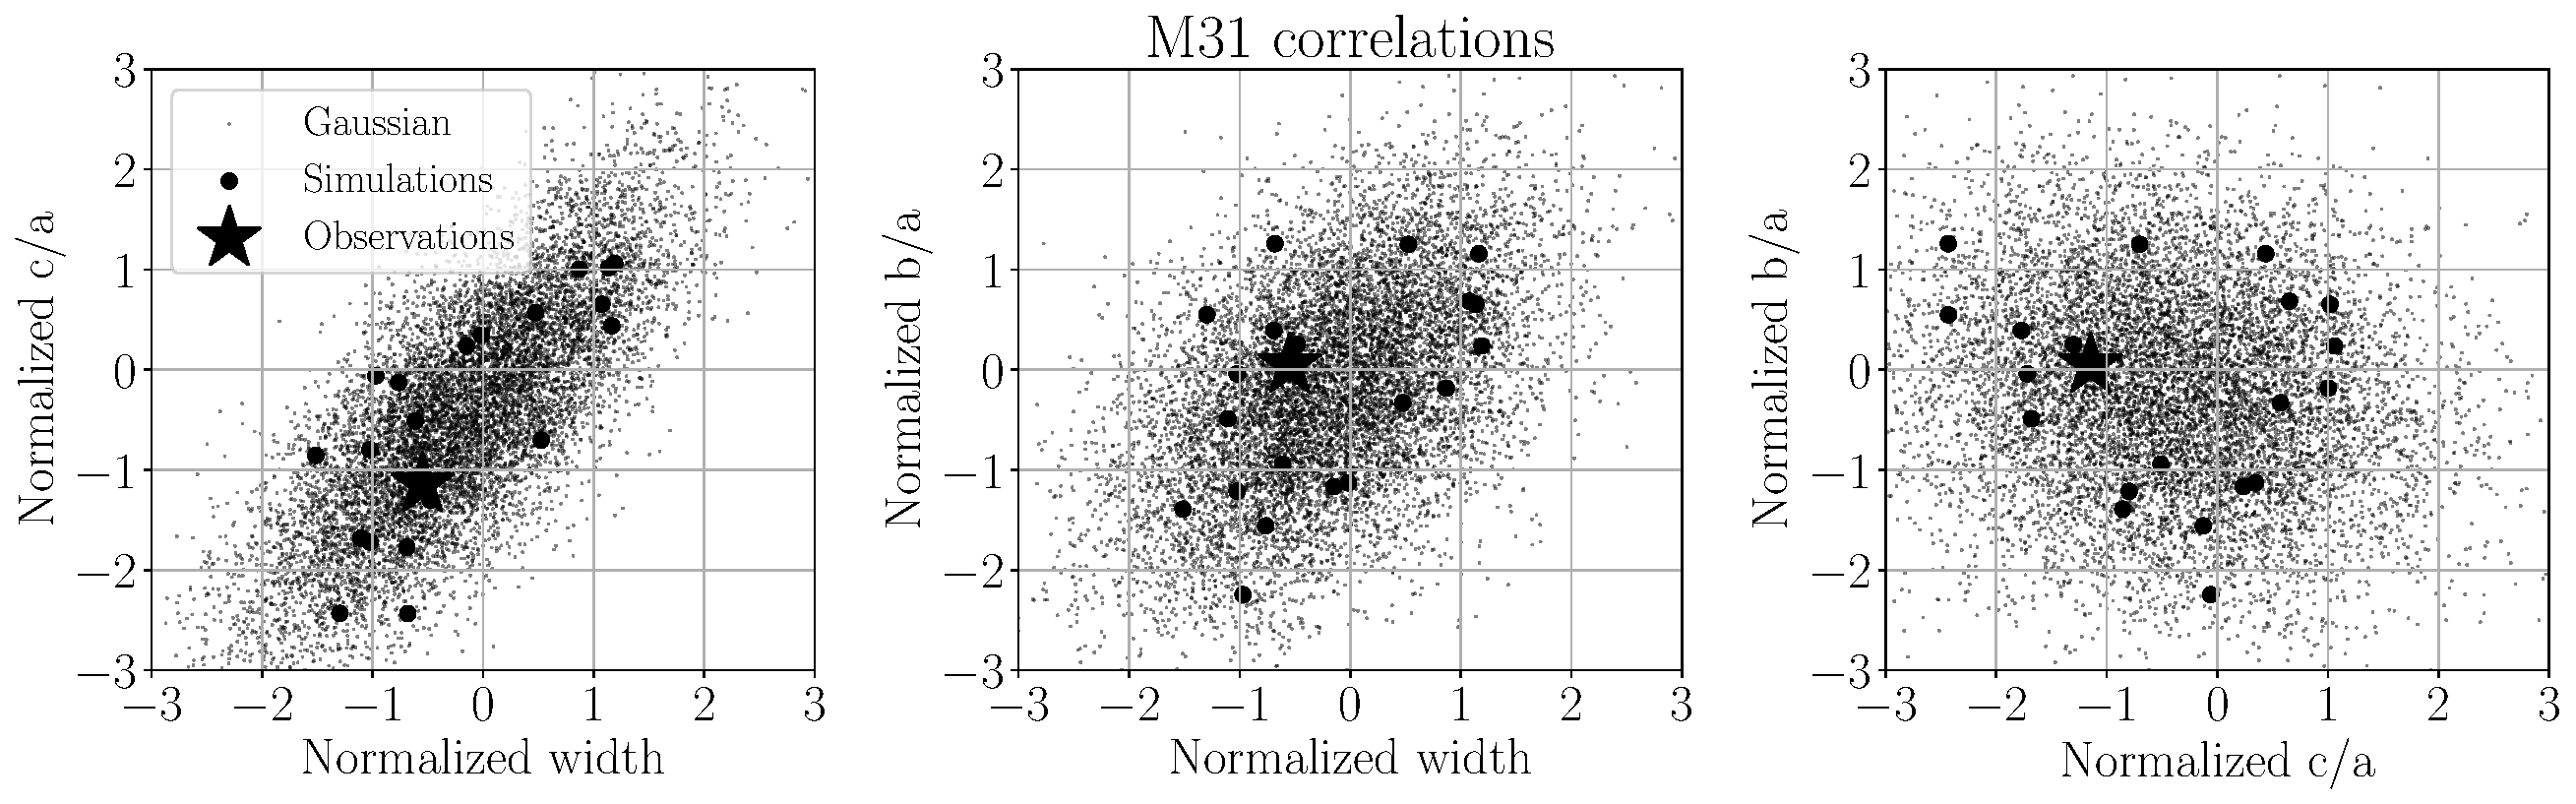
\includegraphics[width=1.0\textwidth]{correlations_M31.pdf}
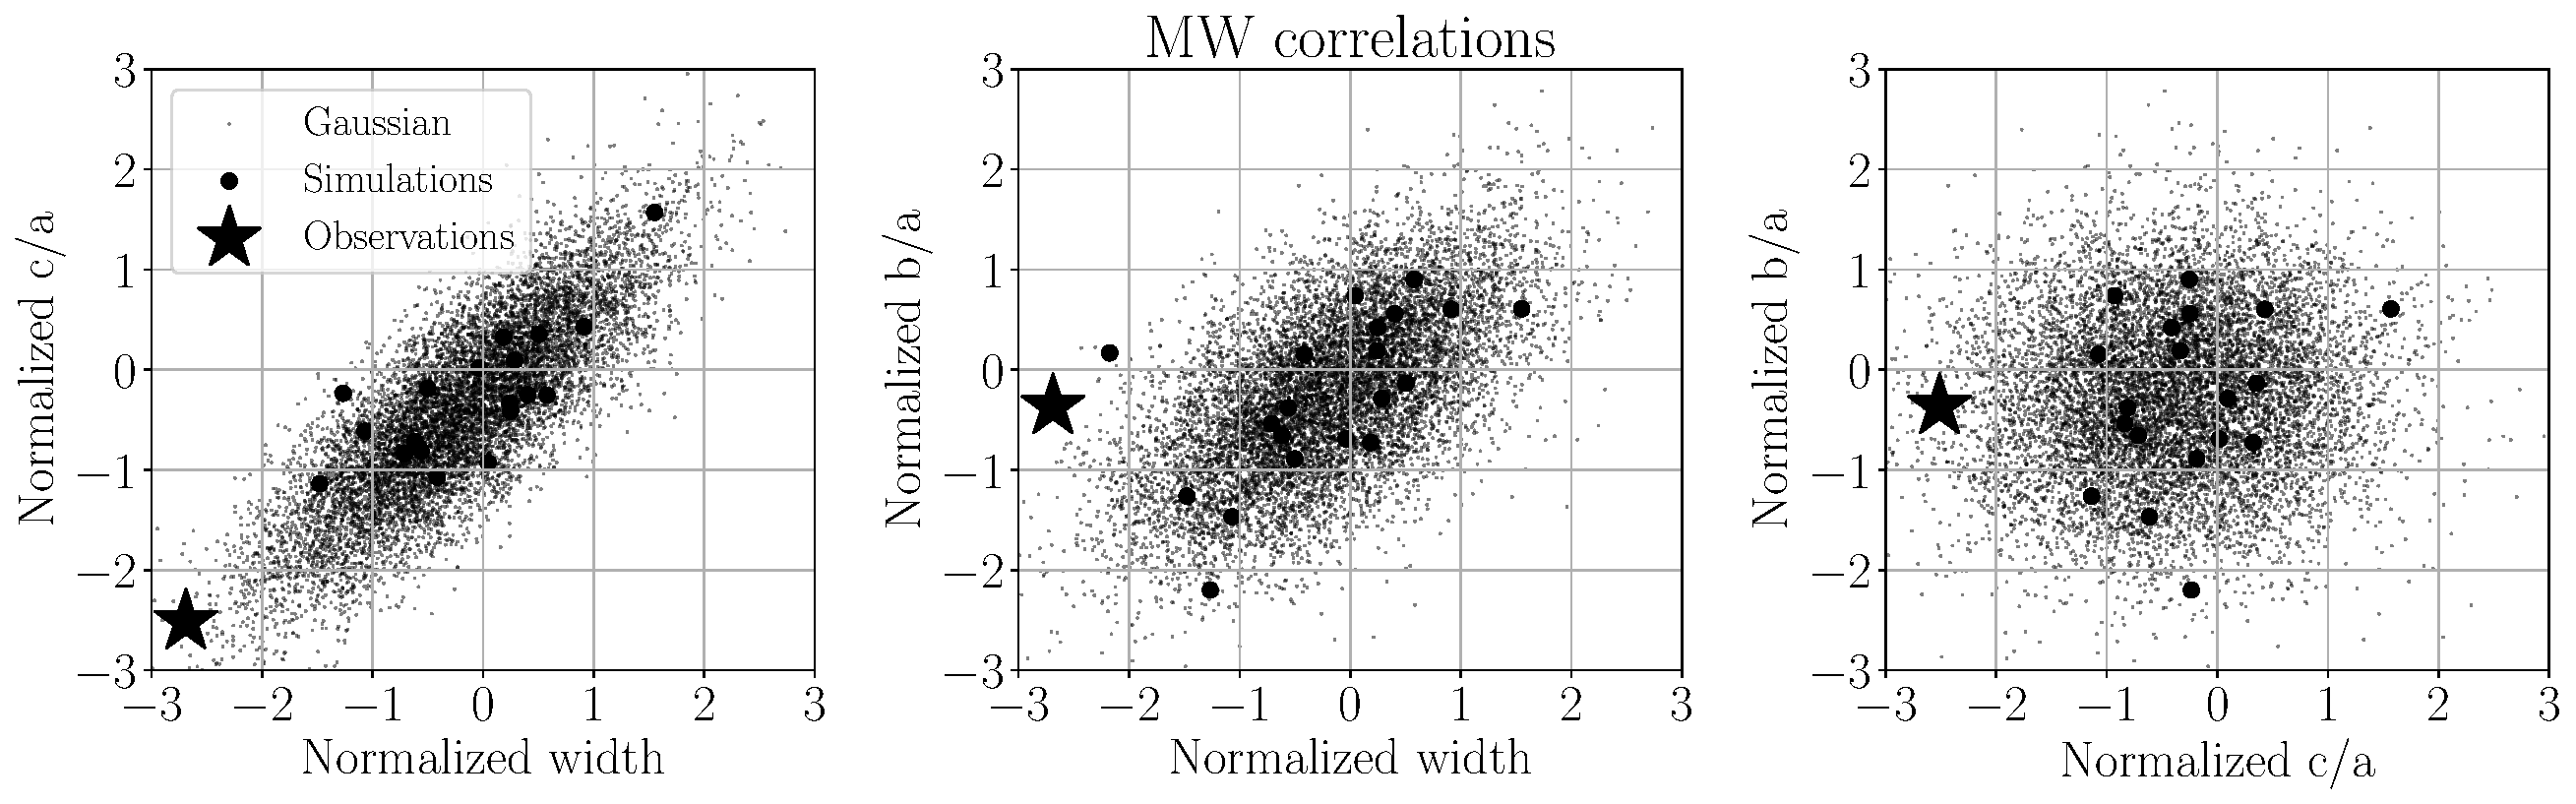
\includegraphics[width=1.0\textwidth]{correlations_MW.pdf}
\caption{Correlations between the normalized values for the plane
  width, $c/a$ ratio and $b/a$ ratio. 
The star corresponds to the LG, black circles with errorbars are the
results from simulations and the gray cloud is the resul from the
multivariate gaussian model.
Upper/lower row summarizes the results for M31/M31.
This simplified description allows us to quantify how atypical is the
LG compared to the simulation results. 
\label{fig:correlations}}
\end{figure*}


\begin{figure}
\centering
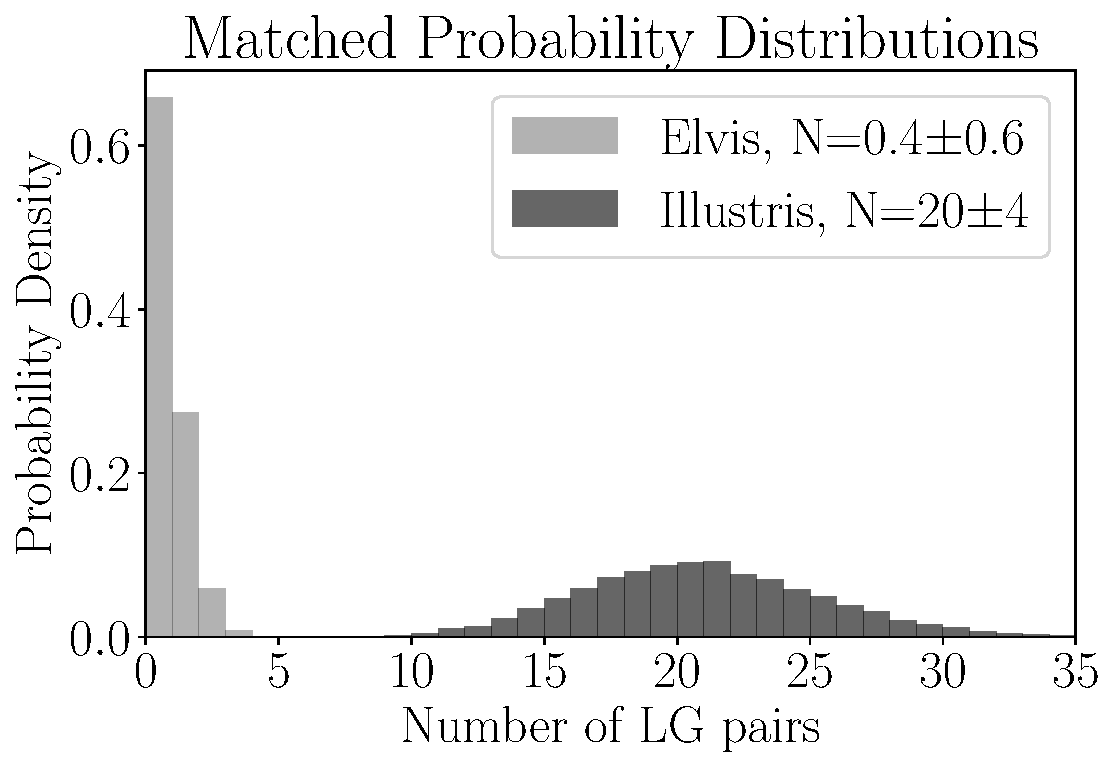
\includegraphics[width=0.47\textwidth]{expected_numbers.pdf}
\caption{Probability distribution for the expected number of pairs
  showing the same degree of atipicality as the Local Group. The two
  distributions correspond to different numbers of initial isolated
  pairs. On average $1\%$ of the isolated pairs should present
  satellite distributions as atypical as the Local Group.
\label{fig:expected_number}}
\end{figure}

\section{Results}
\label{sec:results}


\subsection{Satellite distributions in the Local Group}

Figure \ref{fig:lg_scatter} summarizes our main results for the
observed LG satellite distributions.
We see that the \rank\ and \boot\ samples are consistent 
withing the scatter provided by each sample.
We use the median and standard deviation in each sample to define the
most probable value and its associated uncertaintiy.
This allows us to compare the observational values gainst the
distributions derived from the Illustris simulation.

There is a third sample in Figure \ref{fig:lg_scatter}. 
It corresponds to the set of \rand\ points generated
by randomizing the angular positions of the satellites in each pair in
the \boot\ sample. 
This provides a baseline to understand the importance 
of intrinsic satellite's radial profile distribution in driving the
results.   

The upper left panel in Figure \ref{fig:lg_scatter} shows that the
planar satellite distributions are located perpendicular to the line
connecting the two galaxies. 
It is remarkable that this alignment is almost perfect for both
satellite distributions. 
The points in the \rand\ simply highlights the expected result for a
random angular distribution is a flat distribution in the range
$0\leq\mu\leq 1$.

The upper right panel shows two interesting things. 
First, the MW satellite plane is thiner than its M31
counterpart. 
This is in principle unexepected since M31 is more
massive than the MW and it should have a broader satellite
distribution. 
The second interesting point is that the MW satellite plane is also
thiner than the spherical randomized expectation, while the M31 plane
is right within the expectation of the randomized satellites. 
This is a another piece of evidence showing the highly structured
satellite distribution in the MW in comparison to M31. 
The fact that the \rand\ samples also show a trend towards thinner MW
planes means that the radial satellite distribution in concentrated in
the MW than it is in M31.

The lower left panel re-inforces the picture of a highly structured
MW. 
It corresponds to the $c/a$ ratio and shows the same trends observed
in for the plane width. 
First, the ratio is lower for the MW than it is for M31; second, the
ratio for the MW is also lower than the expectation for the randomized
sample while the results for M31 is within the expectations from \rand.  
In this case the median value of the \rand\ distributions follow the
$1:1$ line as expected.
The lower right panel does not show any surprises. 
All the distributions from \rank, \boot\ and \rand\ are consistent
both for the MW and M31. 

We can quantify the degree at which the observed satellite distributions are 
different from their spherically randomized counterparts.
Figure \ref{fig:lg_distribution} shows the probability distributions
from the \rand\ pairs with an overplot of the LG values.
The upper left panel shows the power law distribution for $\mu$. The
results are not perfectly horizontal because the optimal power value
$\hat{alpha}$ is slightly different from $1$, the uncertainties in
this value are naturally consistent with the unit value expected for
an homogeneous distribution. 
In this case all values are equiprobable.
In the case of the $b/a$ ratio (lower right panel) both the MW and M31
are consistent with the average values expected from \rand\ distribution.
Remarkably, the plane width and $c/a$ ratio for the MW are significantly 
different from the \rand\ expected values, while the M31 values are
sistematically within the expectations.

The comparison of the observed satellite distribution against its onw
version, but spherically randomized, tells us that the MW satellite
planar structure is remarkably different from a random distribution,
while for the M31 distribution there isn't a significant difference
from the random expectation. 

\subsection{Satellite distributions in the Illustris Simulation}

In the previous section we saw how the MW cannot be concealed with its
randomized satellite distribution, while M31 is fully consistent with
it. 
We now quantify whether the MW and M31 are consistent with the
expectations from the Illustris Simulation.
We show here the results from the \rank\ sample. 
The results from the \boot\ sample ara avaialble in the appendix.









\begin{table*}
  \centering
\begin{tabular}{lll}
\hline\hline
Symbol & Units & Description\\\hline
$\hat{r}_{AB}$& & Unit vector along the direction connecting two
dominant galaxies\\
$N_s$ & & Number of satellites\\
$a > b> c$ & kpc & Inertia tensor eigenvalues. \\
$\hat{I}_1$, $\hat{I}_2$, $\hat{I}_3$ & & Inertia tensor eigenvectors. \\
$\sigma_s$ & kpc & Ellipsoid width\\
\hline\hline
\end{tabular}
  \caption{Overview of the parameters computed for each central galaxy
    and its satellite system.
  \label{tab:models}}
\end{table*}

Prospects for observational measurement: DESI.

\bibliographystyle{mnras}
\bibliography{Dwarfs}

%% Alignments between galaxies, satellite systems and haloes
%% https://arxiv.org/pdf/1605.01728.pdf

%M31 mass
%% https://arxiv.org/abs/1410.0017

%MW mass
%https://arxiv.org/abs/1407.1078


\end{document}

